\chapter{Related Works}
\label{chap:RelatedWorks}

In this section we will present a comprehensive review of the state-of-the-art in the field of Vehicle Re-Identification and Single/Multi-Camera Linking. We will start by introducing the general concepts and designs behind re-identification, followed by a detailed analysis of the most relevant works in the literature.

\section{YOLO - You Only Look Once}
Object detection methodologies have undergone several evolutionary phases, all representing the search and the need for more efficient and effective computational vision techniques. Early methods were based on a lot of hand-crafted feature extraction processes that required very intensive human experience and labour.

\textbf{SIFT} \textit{(Scale-Invariant Feature Transform)}, invented by David Lowe in 1999, represented the beginning of a new era in feature detection by constructing scale-space representations, trying to maximize the Difference of Gaussians \textit{(DoG)} in scale and space for identifying keypoints invariant and independent to scaling, rotation and illumination changes. SIFT was able to perform a more robust feature matching across images, which was achieved by convolving the image with a Gaussian filter at different sigma values, where sigma is related to the scale of the filter. By gradually increasing this value, the so-called scale-space representation of the image is obtained and, for each scale, difference of the Gaussian-filtered images is computed to find the DoG, which will clearly highlight regions of rapid intensity change. 

Key points are then found by looking through every point in the DoG representation and comparing it to its neighbors at the same scale, as well as to all of its neighbors in the scale above and below. If a point is a local extrema, in other words it's larger or smaller than all its neighbors, it is marked as a potential keypoint. This ensures that each keypoint is optimally represented at its corresponding scale. In particular, keypoints that have a low contrast or are poorly localized, like keypoints along the edges, are removed according to a pre-computed threshold that enhances the robustness of the detected features. Multi-scale analysis enables SIFT to detect scale-invariant features, significantly enhancing tasks such as object recognition and image matching.

\textbf{HOG} \textit{(Histogram of Oriented Gradients)}, proposed by Navneet Dalal and Bill Triggs in 2005, became one of the most powerful feature descriptors that proved to be very efficient for human detection. HOG calculated the gradient orientation histograms in localized regions of an image with very high accuracy for edge and gradient structure. HOG was able to describe object appearances effectively by dividing images into small connected cells and compiling orientation-based gradient distributions.

The transition to Deep learning marked a paradigmatic shift in object detection methodologies. R-CNN and its successors, Faster R-CNN and Mask R-CNN, introduced learned feature representations to revolutionize the field. These region-based Convolutional Network architectures automated feature extraction, replacing manually engineered descriptors with hierarchical, learned representations.

In \textbf{R-CNN}, the object segmentation pipeline was really slow as RoIs (Region of Interest) were passed to a CNN before applying the final SVM classification, resulting in more than 2000 independent forward passes for each image.

In \textbf{Faster R-CNN}, in particular, authors combined region proposal networks with convolutional feature extractors, thus allowing end-to-end trainable object detection systems that significantly improved accuracy and generalizability, meaning that instead of passing the single cropped images into the classifier, the whole image was given in input to the Convolutional Network, from which the Convolutional Features were extracted and then passed to the Region Proposal Network, which was responsible for generating the RoIs. This approach was much faster and more efficient than the previous one, as it was able to process the whole image in a single forward pass, resulting in 8 hours of training time instead of 84 hours.

In \textbf{Mask-R-CNN}, the authors used a R-CNN which has a mask prediction network that operates on each RoI and predicts a 28x28 binary mask. This mask is then used to extract the features of the object, which are then passed to the classifier. This approach was able to achieve state-of-the-art results in instance segmentation tasks.

Despite these advancements, region-based approaches suffered from computational inefficiencies and substantial inference latency. \textbf{YOLO} \textit{(You Only Look Once)} \cite{YOLO} addressed these limitations by reframing object detection as a unified, single-stage regression problem. By processing entire images in a single forward pass and predicting bounding boxes and class probabilities simultaneously, this model dramatically reduced computational overhead while maintaining competitive detection accuracy.

The algorithm divides the image into an $S \times S$ grid, where an object prediction task is carried out for handling possible objects falling inside that specific cell as shown in Figure \ref{fig:YOLO}. In fact, it then predicts $B$ bounding boxes for each cell, along with their associated confidence scores, which will result in the likelihood that the box contains an object and the accuract of the predicted box's coordinates. Also, conditional class probabilities for each of the object classes, denoted as $C$, are estimated given that the object is in the cell.

% YOLO Image
\begin{figure}[ht]
    \centering
    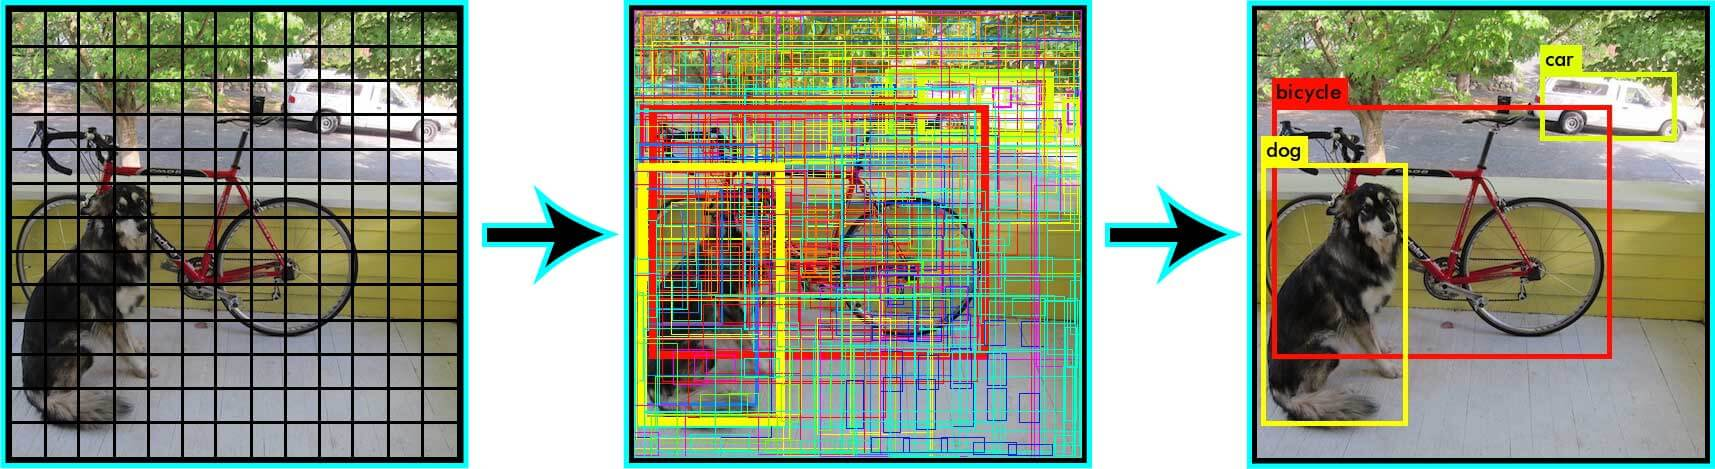
\includegraphics[width=1.0\textwidth]{images/YOLO.jpg}
    \caption[YOLO Object Detection]{Visualization of the YOLO algorithm for Object Detection}
    \label{fig:YOLO}
\end{figure}

One of the major steps in the post-processing pipeline of YOLO is Non-Maximum Suppression (NMS). Here, the goal is to remove all overlapping bounding boxes and keep only the one with the highest confidence score, rejecting redundant boxes with a significant overlap. In its design, YOLO also introduced vector generalization techniques in handling the high-dimensional output tensor, bounding box coordinates, objectness score, and class probabilities. Finally, class scores can be easily converted into probabilities through a simple Softmax function and by the flattening of this tensor into a vector.

Further developments in YOLO brought more complex and optimized architectures and methods to address the weaknesses of the original algorithms, like the detection of small objects, improving localization precision and increasing robustness on diverse visual scenes. More generally, we've seen a great overall evolution of the Object Detection task, starting with the first architectures based on handcrafted feature extractors, SIFT, and HOG, to learning-based region proposal networks, RPN, and from there to real-time, end-to-end detection frameworks that culminated in the architectural innovations of YOLO, which is now a cornerstone for real-time performance with great stability and precision. 

\subsection{YOLOv9}
YOLOv9 represented a major step in the Object Detection field, trying to tackle some of the key challenges around deep learning models with new approaches to information message-passing and network architecture. Its paper introduces two new concepts: Programmable Gradient Information (PGI) and Generalized Efficient Layer Aggregation Network (GELAN), which will revolutionize how Neural Networks handle and retain important information across the many layers of detection.
The heart of the innovation in YOLOv9 is the PGI mechanism, which resolves the long-standing information bottleneck problem of Deep Neural Networks elegantly by providing a reliable way of transporting critical and essential data, ensuring a valid gradient propagation step for more efficient and stable learning. With this, reversible functions for lossless transformations are included in the Network to get dramatic improvements in information retention in deeper architectural layers.
The GELAN architecture, instead, really sets YOLOv9 apart by providing advanced multi-scale feature aggregation, which not only improves the efficiency of parameters, but also enables better detection phases across a wide range of object scales without sacrificing computational efficacy. A result worth of note is given by the fact that the lightweight versions of YOLOv9 (meaning YOLOv9s - YOLOv9c) achieved an higher mAP (Mean Average Precision) on COCO with respect to its precedessor models, considering also the highly reduced computational complexity.
The architectural advances in YOLOv9 make it one of the most important milestones in the history of Object Detection tasks, demonstrating the potential of elaborating network architectures to surmount traditional limitations with gradient flow and feature representation.

\subsection{YOLOv10}
YOLOv10 has been a revolutionary real-time Object Detection system that fundamentally changed the inference process by fully removing Non-Maximum Suppression (NMS), a traditional post-processing technique that has long been a bottleneck in object detection frameworks and which caused a lot of computational overhead and latency, by introducing consistent dual label assignments, achieving a remarkable balance between prediction accuracy and computational efficiency.
The core novelty is a new way of training, in which the authors combined one-to-many and one-to-one assignments. Such a strategy allows the network to provide strong predictions without using heavy complex post-processing mechanisms. Further architectural refinement has been pursued by an elaborately optimized backbone, in which enhanced CSPNet structures improve the flow of gradients while reducing computational redundancy and a one-to-one inference head design is able to generate a single high-confidence prediction per object. This approach and the innovative spatial-channel decoupling techniques, have further streamlined the detection process while reducing the inference latency and computational overhead on a large scale.
Lastly, another key optimization involves the rank-guided blocks that reduce model redundancy while preserving its peak performance. These architectural choices collectively make YOLOv10 one of the most important recent developments in object detection, illustrating how informed design can achieve improvements in accuracy, speed, and computational efficiency all at once.
By reimagining traditional paradigms of detection, YOLOv10 gives a new meaning to real-time object detection and further streamlines visual recognition tasks among researchers and practitioners in a better and more efficient way.

\subsection{YOLOv11}
YOLOv11 has represented another big step in Computer Vision, thanks to its robustness over multiple visual recognition tasks. Its architectural approach achieves a great balance between computational efficiency and comprehensive performance by careful refinement.
The core and major breakthrough resides in the strategic integration of partial self-attention modules, which drastically enhanced the network's capacity to learn a global representation of its sub-tasks. These optimizations allow YOLOv11 to outstand not only in object detection but also in the seamless support of tasks like segmentation, pose estimation and bounding box detection, imposing its architecture as a versatile multi-task solution.
Surprisingly, YOLOv11 achieves these improvements while simultaneously reducing computational complexity. This model shows a 22\% reduction in the number of parameters for its mid-sized variant, YOLO11m, without sacrificing performance but instead improving the mAP across tasks. Large-kernel convolutions play an important role in this optimization, enlarging receptive fields without incurring significant computational penalties.
As already pointed out, the real novelty of YOLOv11 consists in being architecturally flexible, versatile, and seamlessly compatible, from resource-limited edge devices like TPUs to high-performance GPUs and cloud environments. This thereby places YOLOv11 among the most advanced developments within adaptive Computer Vision architectures, setting new standards for computational efficiency in Object Detection tasks. Beyond improving the YOLO series, YOLOv11 definitely set a new frontier for all future multi-use Neural Network designs and architectures in many different applications.

\section{Convolutional Neural Networks}

\subsection{Convolution applied to signals}
Convolutions are among the primary mathematical operations that have been originally introduced in the context of signal processing where they were utilized to analyze and manipulate one-dimensional (1D) signals, which were typically audio waves, electrical signals, or just time-series data, composed of hierarchical, local, shift-invariant patterns.

A convolution is a process involving the sliding of a kernel or filter across an input signal to compute a weighted sum of the signal's local regions, effectively applying transformations like smoothing, sharpening, or edge detection. It enables the analysis of data at a very specific scale while preserving the spatial or temporal relationships, making this operation very powerful in identifying patterns such as frequencies or sudden changes within the signal itself.
A classical signal theory definition, tell us that given two functions $f, g : [-\pi, \pi] \rightarrow R$, their convolution is defined as:
\begin{center}
    \[
        (f * g)(x) = \int_{-\infty}^{\infty} f(\tau) \, g(x - \tau) \, d\tau
    \]
\end{center}
where $(f * g)(x)$ is called Feature Map, while $g(x - \tau)$ is the kernel, which is a function that is applied to the input signal $f(x)$ to extract some specific features.

% Convolution Image
\begin{figure}[ht]
    \centering
    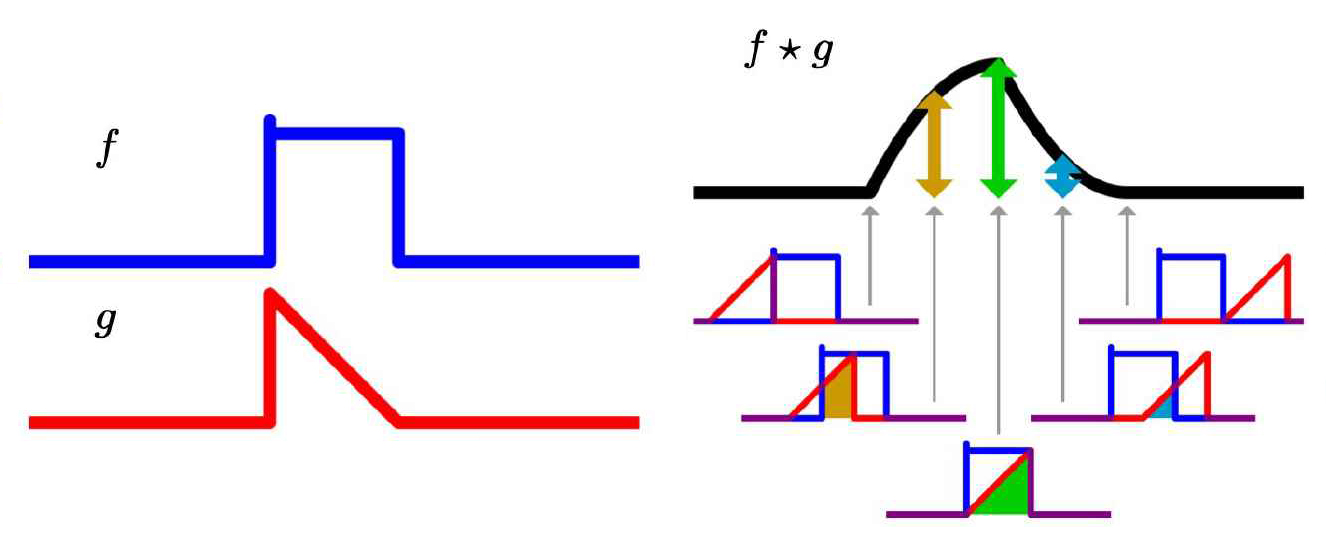
\includegraphics[width=0.8\textwidth]{images/Convolution.jpg}
    \caption[Convolution operation applied on a signal]{Convolution operation applied to a signal}
    \label{fig:Convolution}
\end{figure}

or either, a lesser known definition via Discrete Time Convolution, where given two vectors $x$ and $w$, we define the Convolution as:

\begin{center}
    \[
        (x * w)_{i} = \sum_{k=0}^{n-1} w_{i-k \, \text{mod} \, n} \, x_k
    \]
\end{center}

In this situation, the convolution operation can be computed in two ways:
\begin{itemize}
    \item As a Circulant Matrix denoted as $C(w)$ which is applied to $x$ in the original spatial domain. $C(w)$ carries a special structure as it's formed by stacking shifted (\textit{modulo n}) versions of $w$. Also, in general, a particular choice of $w$, like $[0, 1, 0, ..., 0]$ or $[0, 0, 1, ..., 0]$ yields a special Circulant Matrix that shifts those vectors to the right by one position as $y = S \cdot x$, where $S$ is this Shift Matrix.
    \item In the Fourier basis, also called Spectral or Frequency Domain, by first computing the Fourier transform of $\phi^{*}(x)$ and multiplying it by the Fourier transform of $w$ and, finally, computing the Inverse Fourier transform of $\phi = \phi^{-1}$.

    Mathematically speaking:
    \[
        (x * w) = \phi^{-1}(\phi^{*}(x) \cdot \phi^{*}(w))
    \]
\end{itemize}

\subsection{Applying Convolutions to Neural Networks}
As the understanding of this concept developed, researchers recognized that these Convolutions could be effectively utilized not only for one-dimensional (1D) signals but also for two-dimensional (2D) data, including images, using two-dimensional filters. The mathematical representation remains largely consistent with that of the one-dimensional scenario. However, the kernel is now represented as a matrix, while the input signal takes the form of a 2D image.

\begin{center}
    \[
        (f * g)[x, y] = \sum_{i} \sum_{j} f[i, j] \cdot g[x - i, y - j]
    \]
\end{center}

The convolution operation is carried out by sliding the Convolutional Filter $g$ (also known as Convolutional Kernel) over the image, computing the dot product of the kernel and the local patch of the image at each location $[x, y]$, thus producing a feature map. This operation is then applied iteratively for every point in the image, resulting in a transformed image that enhances the presence of the extracted features (edges, corners, and textures), capturing the local patterns of the image.

Furthermore, there might be cases in which the Convolutional Kernel can be directly applied on top of the image or can't be applied because it would exceed the image boundaries. This cases are visually represented in Figure \ref{fig:Padding} and listed below:
\begin{itemize}
    \item Valid Padding: Also known as \textit{No Padding}, it is a scenario where the convolution kernel is directly applied to the boundaries of the underlying function, and hence, the output image size turns out to be smaller than the input image size. Its output dimension is $O = D - N + 1$ for an input dimension $D$ and kernel dimension $N$.
    \item Same Padding: Also known as \textit{Zero Padding}, it pads the input image with zero vectors to increase the size of the image borders, so that the kernel could be applied on the complete image. The output image thus obtained will have a size equal to that of the input image. Such padding gives an output size $D$, where $D$ is the input size.
\end{itemize}

The domain, in some cases, may be dilated and padded with zeros, but such padding may still not be enough to provide a good fit for the boundary pixels. Therefore, an arbitrary and tunable Stride value may be used in moving the kernel over the image. Stride is the number of pixels that the kernel is moved over the image, and it may take any value, although it is usually set to 1.

% Padding Image
\begin{figure}[ht!]
    \centering
    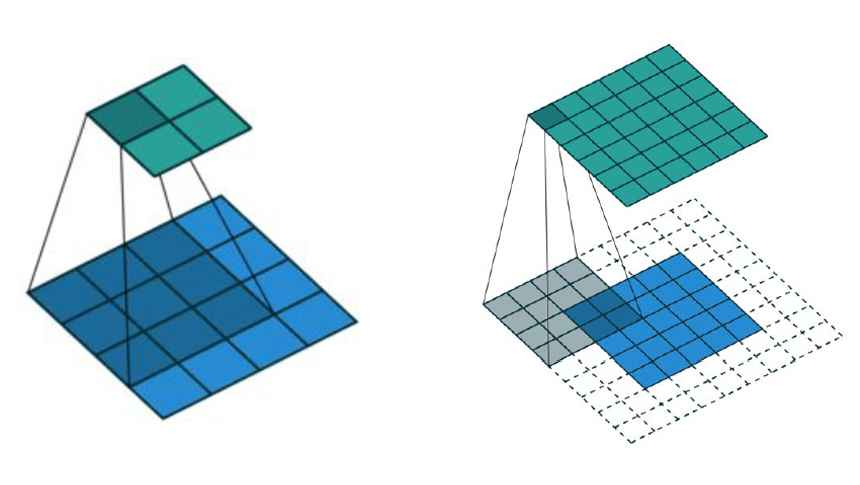
\includegraphics[width=0.8\textwidth]{images/Padding.jpg}
    \caption[Padding algorithms]{Valid padding (on the left) and Same padding (on the right) applied on top of a 2D image}
    \label{fig:Padding}
\end{figure}

This served as a starting point for applying convolutional operations to Computer Vision tasks, allowing the model to understand visual information with spatial hierarchies. The key transition from traditional signal processing to CNNs occurred when these filters were incorporated into Neural Network architectures in which their parameters could be learned in an automated manner during training. This change allowed for the automatic discovery of task-specific features, going beyond handcrafted filters to dynamically and automatically optimized convolutional filters.
The first Convolutional Neural Networks (CNNs) were designed for processing 1D signals, such as audio waves or time-series data, by applying 1D convolutions to extract hierarchical, local, shift-invariant patterns. Generally speaking, the i-th Hidden Unit $h_i$ in a CNN is computed as the convolution of the input signal $x$ with a filter $w_i$ and a bias term $\beta$, followed by a non-linear activation function $\alpha$:

\begin{center}
    \[
        h_i = \alpha \cdot [\beta + \sum_{j=1}^{n} w_{j} \cdot x_{i+j-2}]
    \]
\end{center}

Researchers, as previously explicated, tried to exploit the power of Convolutions to process 2D data, such as images, by applying 2D convolutions to extract features from the images. That's where these so-called Convolutional Neural Networks, or CNNs for short, were initiated, a type of Deep Learning architecture very well suited for the interpretation of visual images. CNNs work in a sequential manner, meaning that they first use Convolutional Layers for extracting hierarchical patterns and features from the input image, Pooling Layers for downsampling the feature maps, thus reducing its spatial dimensions and, finally, Dense Layers to output strong embeddings, as shown in Figure \ref{fig:CNNArchitecture}.

% CNN Architecture
\begin{figure}[ht]
    \centering
    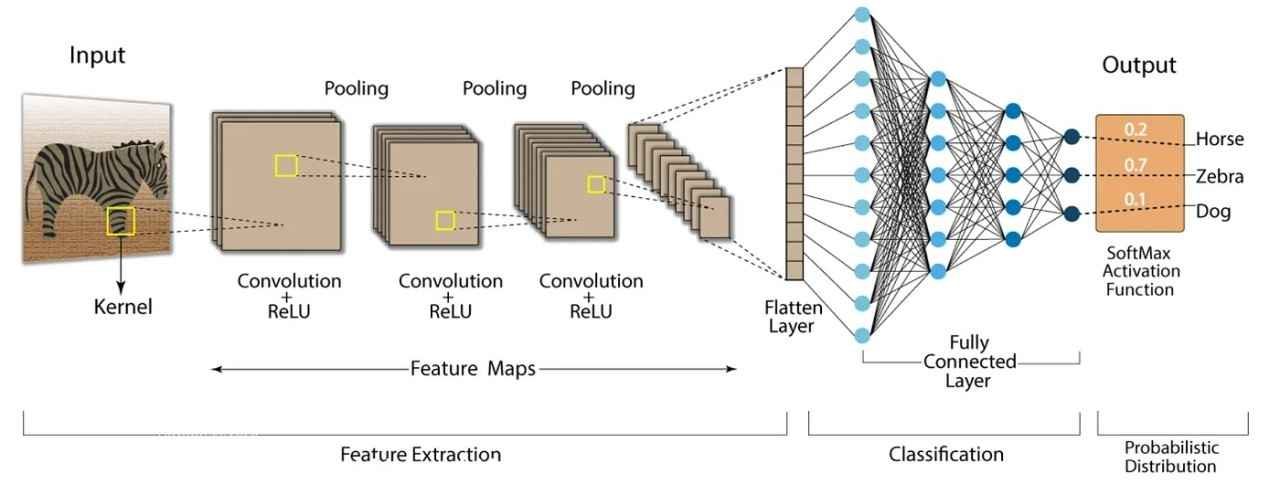
\includegraphics[width=1.0\textwidth]{images/CNN Architecture.jpg}
    \caption[A common CNN architecture]{A typical Convolutional Neural Network (CNN) architecture}
    \label{fig:CNNArchitecture}
\end{figure}

Furthermore, as visually represented in Figure \ref{fig:CNNFeatures}, the initial layers of the Convolutional Layers perform low-level feature extraction such as edges, corners, and textures. The middle layers extract more complex features, which could be shapes and patterns, while the final layers extract high-level features, which could be objects and scenes. The last Dense Layers are responsible for generating the last embeddings, thanks to which the classification of the input image can fall under a given class. The output from the Dense Layers is then passed through a Softmax function, which converts this output into probabilities to help identify the input image under one of the defined classes.

% CNN Features Image
\begin{figure}[ht]
    \centering
    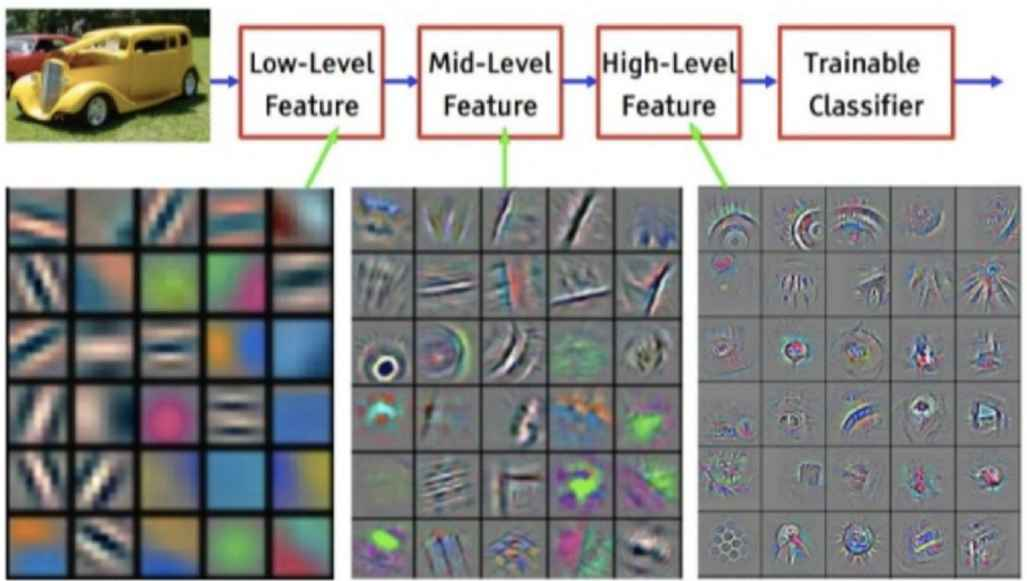
\includegraphics[width=0.8\textwidth]{images/CNN Features.jpg}
    \caption[CNN feature extraction process]{CNN features extraction process}
    \label{fig:CNNFeatures}
\end{figure}

The evolution of the field from signal processing to learned representations in Neural Networks changed fields like Computer Vision and laid the bedrock for advanced architectures, such as ResNet or VGG, using Convolutions for deep hierarchical feature extraction and hence overcoming problems like vanishing gradients and overfitting.

\subsection{ResNet}
Generally speaking, a Neural Network is nothing else than a sequential composition of layers, where each layer is a function that takes an input and produces an output which is then passed as input to the next layer, and so on and so forth. Equivalently, since this processing is sequential, its output $y$ can be seen as as series of nested functions:
\begin{center}
    \[
        y = f_{4}\,[f_{3}\,[f_{2}\,[f_{1}[x, \phi_{1}],\,\phi_{2}],\,\phi_{3}],\,\phi_{4}]
    \]
\end{center}

ResNet \cite{ResNet} is a special type of Convolutional Neural Network (CNN) where the authors introduced the concept of \textbf{Residual Connections}, an architectural contribution that has revolutionized the field of Deep Learning. These connections allow layers to learn residual functions with respect to the inputs of previous layers, which significantly increases the trainability of Deep Neural Networks.
While in standard neural networks, the layers aim to directly construct the mapping $H(x)$ from the input $x$ to the output $y$, ResNet reformulates the problem by letting the layers learn a residual mapping $F(x) = H(x) - x$, so that the original mapping becomes $H(x) = F(x) + x$. This simple yet effective strategy has major implications for the design and optimization of deep networks.

Here, the output of the layer is the summation of the input that is fed into the layer and its own output, which is passed through a non-linear activation function. This way, the Network will be able to learn residual functions, which are much easier to optimize, hence overcoming the problem of vanishing gradients.
This is a phenomenon that occurs when the gradients of the loss function decay drastically during their backpropagation through the network, which might slow down the network's capability to learn optimal weights in very deep architectures. With the direct reintegration of the input into subsequent layers via residual connections, the gradient signal remains at a strong level, thus training at high speed—even with hundreds of layers—can be realized for the networks.

A generic Residual block is composed as follows:
\begin{center} 
    \[
        y = f(x) + x
    \]
\end{center}

The operation denoted by $+ \, x$ is facilitated via a \textit{skip connection}, which implements an identity mapping by establishing a straight connection between the input and output of the subnetwork. This is referred to in literature later as a \textit{residual connection}, also shown in Figure \ref{fig:SkipConnection}. Here, the function $F(x)$ usually consists of matrix multiplication interlaced with activation functions and normalization processes, such as batch normalization or layer normalization. Collectively, these components form the so-called \textit{residual block} which is a primary building block of ResNet. By stacking many residual blocks, one may construct a deep residual network that has the ability to efficiently solve complex learning problems.

% Skip Connection Image
\begin{figure}[ht]
    \centering
    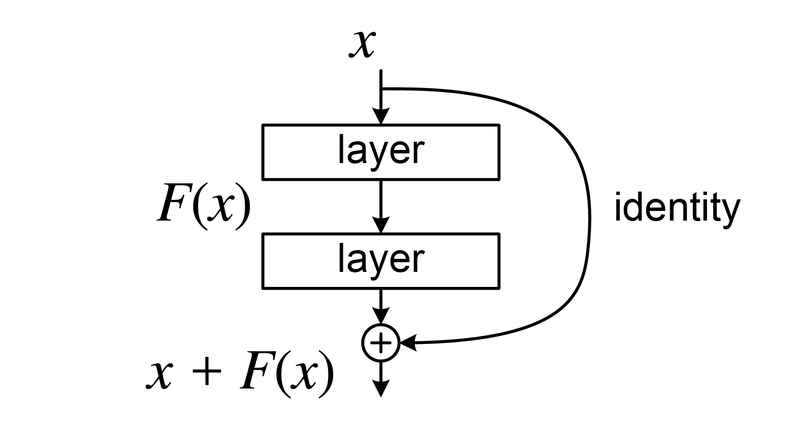
\includegraphics[width=0.5\textwidth]{images/SkipConnection.jpg}
    \caption[A skip-connection strategy]{A skip connection strategy}
    \label{fig:SkipConnection}
\end{figure}

What makes ResNet important is not the architecture itself, but rather the use of Residual Connections, which provides greater flexibility, enabling the network to deepen without the risk of performance degradation, simply known as the degradation problem.

Without such connections, more complex networks might perform worse than simpler ones because of the difficulty in arriving at meaningful solutions. ResNet alleviates this by ensuring that at the very least, even if additional layers aren't improving the network's performance, they won't hurt it either, since via residual learning, those layers can learn to approximate an identity function if there is need to. Furthermore, ResNet blocks allow large-scale features and smaller-scale adjustments to be learned in separate ways. The very first layers, as depicted in Figure \ref{fig:ResNet}, learn very general and broad features, while much deeper layers focus on details. By introducing residual connections, these deeper layers are able to focus on improving the outputs of the earlier layers, rather than having to relearn these features from scratch. Such hierarchical refinement is particularly useful in tasks such as Vehicle Re-Identification, where subtle differences between vehicles need to be well captured.

% ResNet Architecture Image
\begin{figure}[ht]
    \centering
    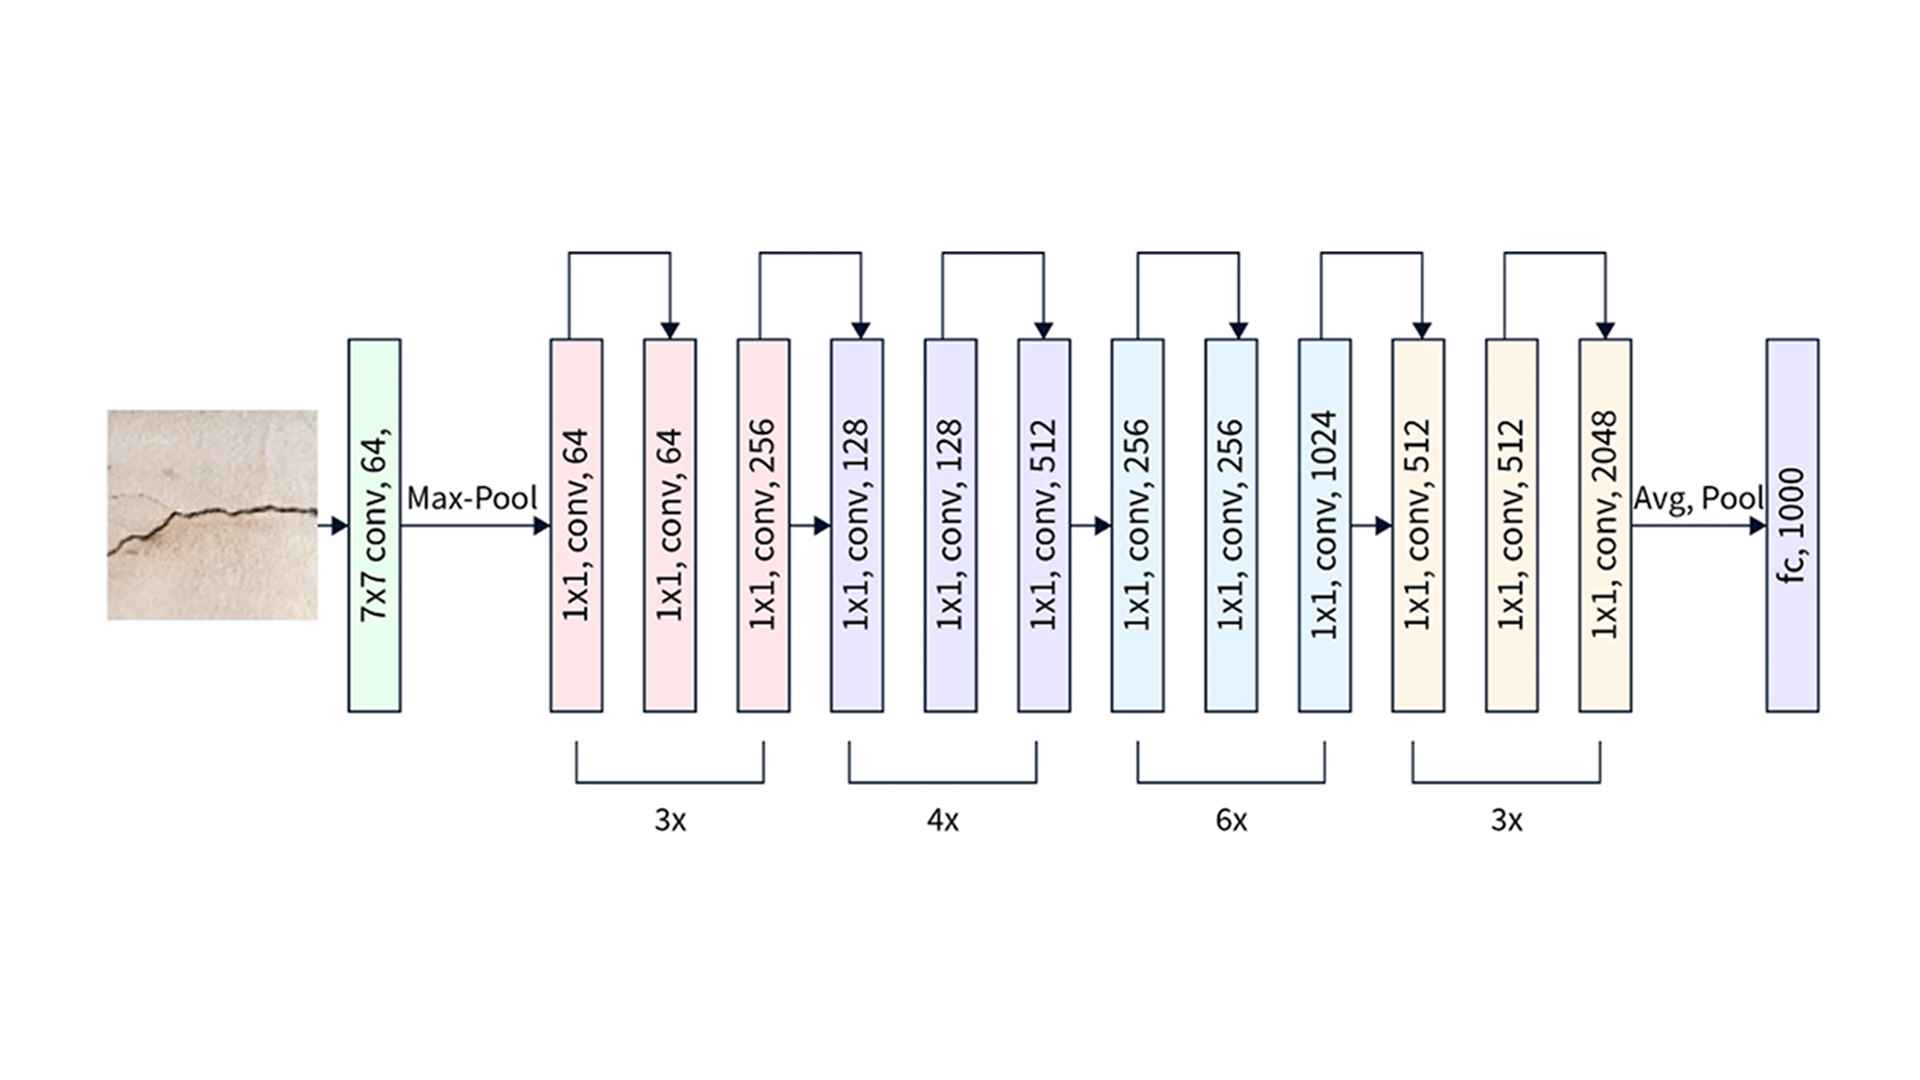
\includegraphics[width=1.0\textwidth]{images/ResNet.jpg}
    \caption[ResNet architecture]{A complete ResNet architecture}
    \label{fig:ResNet}
\end{figure}

Another major benefit of this residual architecture is its suitability and versatility for transfer learning, a very important method in tasks like Vehicle Re-Identification. Pretrained ResNet models, trained on huge datasets like ImageNet, are fine-tuned for specific tasks in a domain with very few modifications because the residual connections preserve the flexibility and effectiveness of the feature extraction for different tasks.

The wide adoption of ResNet has inspired many derivatives and extensions, including ResNeXt, Wide ResNet, and DenseNet, which expand the basic idea of residual connections to improve performance and efficiency. ResNet remains one of the most essential components of deep learning and is currently a principal architectural framework used in many state-of-the-art Vehicle Re-Identification systems due to its flexibility and robustness.

\subsection{ResNeXt}
ResNeXt \cite{ResNeXt}, for the first time introduced in November 2016, is the evolution of the ResNet architecture, introducing the concept of cardinality, which refers to the number of independent paths taken to process the input. In this new design, a modular approach is introduced where multiple parallel transformations are aggregated to form the final output. Unlike traditional ResNets, which seek better performance by increasing the depth or width of the network, ResNeXt improves accuracy, on complex datasets such as ImageNet, by increasing cardinality, that is, the number of sets of transformations aggregated in each residual block which enables the model to represent more diverse features, hence increasing the accuracy of classification. All these paths have the same topology, preserving architectural simplicity while increasing the representational power of the Network.

ResNeXt blocks introduce grouped convolutions as an effective mechanism that splits input channels into groups and performs independent convolutions in each one of them, thus managing to keep computational efficiency and increasing the expressive power of the network, along with a new dimension for optimization. A key advantage of this design is that the accuracy scales well without considerable additional computational complexity or a great number of parameters, as indicated by the fact that ResNeXt outperforms ResNet with a similar model size and FLOPs.

Conclusively, as per its paper, ResNeXt outperforms ResNet in a number of different tasks, such as object detection and segmentation, even if it retains some of the core foundations of the base model, placing it as one of the most powerful architectures for leading state-of-the-art Computer Vision performances.

\section{Global and Local Features}
\subsection{Limitations}
In the early years of research on this exciting topic, most efforts were given on license plate-based methods, trying to rely entirely on automatic plate-based recognition techniques \cite{LicensePlate_1, LicensePlate_2}, which emphasized the identification of vehicles according to textual and structural features of the license plates themselves. Under some conditions, these methods performed fine, but limitations were really evident. License plates could be easily occluded, intentionally changed, or being invisible due to environmental conditions or camera placement. For example, top-view camera installations, used mainly in real-world surveillance, hardly ever catch the license plate details. All these drawbacks led to a shift in focus by researchers towards vehicle appearance-based methods, which are more robust and keen to overcome these problems and where visual features of the vehicle rather than the license plate alone were used.

\subsection{Appearance-based models}
Appearance-based models, then, have since become a powerful alternative by leveraging the higher-level visual characteristics of vehicles such as shape, color and texture, in order to form discriminative representations. However, most pure CNNs poorly succeed in encoding those fine-grained details, which are critical for Vehicle Re-ID, because they do tend to rely more on global features, overlooking some local subtle features, discriminative as well, like inspection marks, small ornaments and unique car design patterns which might distinguish one car from another. These fine-grained details are of great importance for the solution of the basic problems of Vehicle Re-ID: large intra-class variations and small inter-class differences as shown in Figure \ref{fig:IntraInterClass}.

For this reason, authors have been trying to take it one step further by directly working on global features, local features and also a mix of them. 

The work by H. Chen al. in \cite{VehicleReID_3} involves improving the discriminative ability of vehicle appearance signatures via a two-branch architecture, \textbf{Partition and Reunion Network} (PRN). The model partitions the feature maps in a three-dimensional way to obtain more robust local features along the height, width, and channel dimensions simultaneously, so as to handle the high visual similarities among vehicles thanks to its partitioned architecture composed by two independent branches: the Height-Channel and Width-Channel branch. These branches deal with height-wise and width-wise partitioning, respectively, where non-redudant spatial features are kept. Each of the partitioned feature maps is then processed through Global Max Pooling, followed by dimensional reduction and normalization layers, to produce feature vectors that are finally concatenated into a complete appearance signature.
The PRN framework proportionally balances the local specificity and global context, which empowers it to be a strong vehicle re-identification tool in complicated scenarios.

In \cite{VehicleReID_1}, J. Zhu et al. proposed a novel approach for merging both the global and local features of the vehicles in order to improve the performance of the Vehicle Re-ID methods, introducing the concept of \textbf{Quadruple Directional Deep Learning Features} (QD-DLF), by exploiting the four directional pooling layers in such a way that the features should become not only robust but also very discriminative when describing vehicular images. These layers help encode different spatial information, so the method becomes more robust under viewpoint changes.
The QD-DLF method is based on a densely connected Convolutional Network that first extracts basic feature maps, further processed by the directional pooling layers. The resulting directional features are normalized and clustered together to properly construct a representation of the vehicle. Particularly, this approach tackles one of the largest challenges in vehicle ReID—viewpoint variations—since it effectively captures the features that remain constant from one camera to another. 

Meanwhile, in \cite{VehicleReID_2}, J. Qian et al., proposed a new framework for specifically solving the problem of how to distinguish visually similar vehicles. The authors introduce a two-branch CNN, named \textbf{Stripe-based and Attribute-aware Network} (SAN), which embeds complementary feature extraction strategies. The first branch of the Network, called the Stripe-based branch, is designed to extract part-level features using horizontal Average Pooling and Convolutional layers. In this way, the network could obtain small-scale details about specific regions in a vehicle, which may include inspection marks or unique decorations used in distinguishing between vehicles that otherwise have similar appearances.
The second branch is the Attribute-aware branch, which further refines the global feature extraction of the network with the help of vehicle attribute labels in training. This ensures that a vehicle with different attribute labels will be well separated even if their overall visual appearances look alike.
The proposed network concatenates the part-level features from the Stripe-based branch with the global features from the Attribute-aware branch in order to generate a unified and highly discriminative descriptor for each vehicle. It also combines local and global information, which tackles the key challenges in vehicle re-identification and enhances the robustness of this task applied to real-world scenarios.

Further work and research introduced the so-called \textbf{IBN-Net} \cite{IBN-Net}, a novel architecture which, for the first time, combines the strengths of Neural Networks such as ResNet, SENet, etc. with normalization techniques like Batch Normalization (BN) and Instance Normalization (IN) as building blocks. This integration enhances the feature extraction capabilities of robust networks like ResNet while leveraging BN and IN to address the internal covariate shift, thereby improving both training efficiency and overall performance. Consequently, state-of-the-art results have been achieved by ResNet-IBN, significantly enhancing the mAP on VeRi-776, a very well-acknowledged large-scale benchmark dataset for Vehicle Re-ID.

\section{Single \& Multi-Camera Tracking}

\subsection{Tracker}
As stated, re-identification of vehicles is a crucial task when multiple cameras are deployed, since establishing the correspondence of a single vehicle from different viewpoints requires exact temporal and spatial alignment. Recently, algorithms have been proposed to handle the issues of object tracking. Among these, SORT (Simple Online and Realtime Tracking) \cite{SORT} and its improved version, DeepSORT \cite{DeepSORT}, are highlighted for their balance between accuracy and computational efficiency.

% Tracker Image
\begin{figure}[ht]
    \centering
    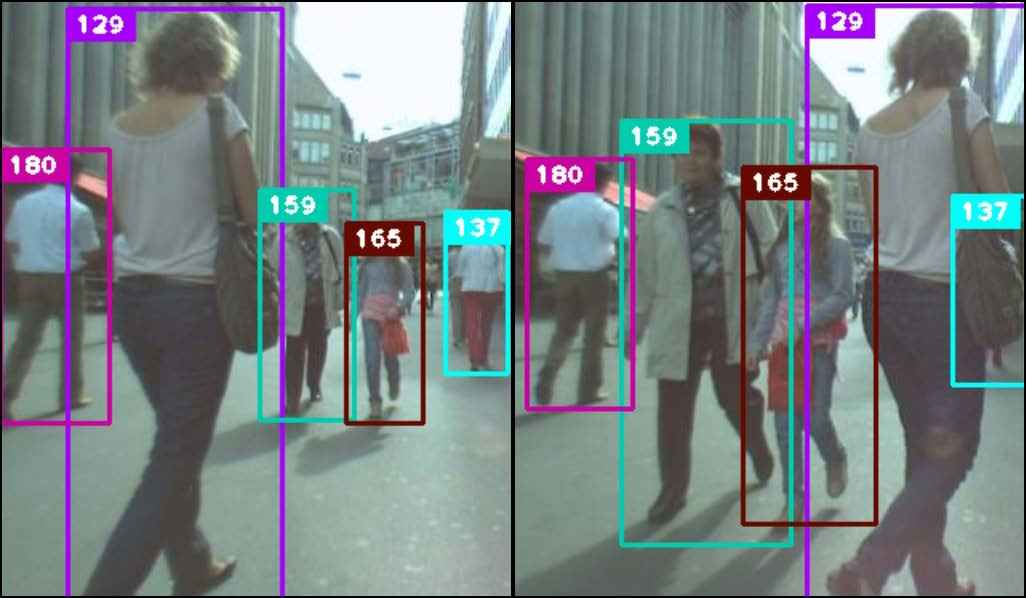
\includegraphics[width=0.8\textwidth]{images/DeepSORT.jpg}
    \caption[DeepSORT Tracker example]{DeepSORT tracker successfully handling occlusions in a MOT challenge scenario}
    \label{fig:DeepSORT}
\end{figure}

Speaking of \textbf{SORT}, the authors developed a lightweight and practical association framework to tackle the issue of tracking-by-detection, designed expressly for real-time Multiple Object Tracking (MOT or MTSC). The framework is focused on efficiency by merely concentrating on the data association between successive frames without delving into the computational complexities of appearance modeling. This makes SORT particularly applicable for tasks that require real-time output, such as autonomous driving or pedestrian observation.
The basic building block of SORT is a combination of standard techniques. The motion estimation is made using a constant velocity linear model, where the position, velocity, scale and aspect ratio of each object are predicted using a Kalman Filter. This makes the model very robust to propagate the states of the objects across frames. The intersection-over-union (also denoted as IoU) between predicted bounding boxes and the new detections are computed by SORT to be able to associate the latter with already existing tracks. The Hungarian algorithm is then used to solve the data association problem optimally, ensuring correct one-to-one matches between detections and tracks. A minimum IoU threshold is applied to discard poor matches, which also implicitly handles short-term occlusions. In order to manage the lifecycle of the tracked objects, SORT initializes new trackers for unmatched detections and terminates those existing ones that do not get updated for a predefined number of frames. This approach guarantees computational efficiency, simultaneously preserving the reliability of the tracker.
SORT is realized in a tracking-by-detection paradigm, paired with object detectors like Faster R-CNN to achieve precise bounding boxes. In contrast to most other tracking systems, SORT does not use appearance-based re-identification and relies solely on geometric information to conduct stable tracking. Although this reduced architecture complexity, it may not deal with longer occlusions or re-identify objects that move out and later come back into the field of view.
For this reason, SORT has achieved a significant MOTA score of 33.4 on the MOT benchmark, outperforming many more complex online tracking systems. Its simple design also enabled it to operate at an outstanding speed of 260 frames per second using a single CPU core, placing it among the fastest tracking solutions available today.

\textbf{DeepSORT} is an extension of the SORT framework in order to overcome the previously specified weaknesses by integrating appearance-based data association into the tracking procedure. Unlike SORT, which relies solely on motion modeling by Kalman filtering and the overlap of bounding boxes (IoU) for data association, DeepSORT uses a deep learning-based appearance descriptor to improve robustness, especially for scenarios with occlusions, re-identifications, and visually similar objects, as can be seen in Figure \ref{fig:DeepSORT}.
The key idea behind this method is to include a Deep Convolutional Neural Network (CNN) trained on a large-scale person re-identification dataset that generates unique appearance embeddings for each detected object. These are then normalized to the unit hypersphere and stored as a gallery of recent appearance descriptors belonging to each track. Data association then proceeds as a combination of motion-and appearance-based measures. Particularly, the Mahalanobis distance obtained with SORT is retained to embrace motion consistency, while the cosine distance between appearance embeddings is added to represent the visual similarity. The aggregation of such metrics via weighted sum determines the final association cost, thus striking a balance between spatial coherence and appearance similarity.
DeepSORT addresses challenges raised by its counterpart SORT, such as object tracking during occlusion, by using appearance embeddings to restore object identities after short-term invisibility. Then, a matching cascade takes place, which gives a preference to the tracks more recently updated. In this way, the tracker's capability in handling long-term occlusion gets definitely improved. Tracks that find no match in any detection are marked as unconfirmed and removed if no match is found within a given timeframe. This helps to increase stability and reduces the number of identity switches (IDs).
Evaluation on the MOT benchmark demonstrates that DeepSORT reduces those identity switches by about 45\% compared to SORT while maintaining competitive tracking accuracy and real-time performance. The system runs at 20 frames per second on modern GPUs, even with such added complexity from the feature extraction, and thus can be applied in practical scenarios. By fusing motion and appearance cues, DeepSORT significantly pushes the state of online tracking and closes the gap between accuracy and efficiency.

\subsection{Trajectory Clustering}
Trajectory clustering is a fundamental aspect in MTMC systems, since it links vehicle tracklets across different camera views. Most of the recent works, rooted in the concepts of detection and tracking, have come up with methodologies that depend on the clustering of tracklets using temporal, spatial, and visual information to accurately associate the tracks across a widespread network of cameras. Many of these approaches combine motion models, temporal constraints, and re-identification features to refine the calculations of tracklet similarity.

One of the methods used by Liu C. et al. in \cite{CityScaleMTMC}, aims at grouping tracklets by their spatial closeness and temporal synchronization, applying methods such as filtration of static or incomplete tracklets to reduce noise and irrelevant information. These filtration methods ensure that only meaningful tracklets with valid motion are considered. Constraint of directionality and timestamps further refines the process of clustering.

Another alternative \cite{OcclusionAwareMTMCT}, enhances this process through the use of scene topology and occlusion awareness, from which their system is able to to remove those tracklets that are unlikely to be linked to the same vehicle. Furthermore, occlusion-aware strategies improve the feature extraction step by removing bounding boxes affected by overlaps or background noise, ensuring that the extracted visual features are reliable and truly representative of the vehicles.

The clustering methodologies provide the core structure of Multi-Camera Tracking Systems because they fuse robust trajectory filtering, temporal alignment, and scene modeling for accurate tracklet association within a complex camera network.
